\section{Methodology}
\subsection{Data Collection and Description}
We used data from XWiki, an open-source wiki platform. From their website, we scraped a dataset of 1,600 manual test cases and 52,860 test executions. Each test case is structured with a description, title, steps to reproduce, and expected results. For instance, a typical test case might look like this:

\begin{Verbatim}[fontsize=\small]
    "https://test.xwiki.org/xwiki/bin/view/File%20Manager%20Tests/Delete%20a%20file": {
        "title": "Delete a file",
        "steps_to_reproduce": [
            "Click on File Manager from Applications Panel",
            "Click on All Files",
            "Select a file",
            "Click on Delete",
            "Click on OK"
        ],
        "expected_result": [
            "The file is deleted."
        ]
    }
\end{Verbatim}

The dataset chosen for this study is especially fitting for us because it contains detailed textual descriptions in the form of test steps. These descriptions can help determine the similarity between tests, which we can use to cluster them together.

\subsection{\ac{NLP} Techniques and Test Selection Process}

To find similar test cases, we use a mix of text embedding and clustering. The approach to finding similar test cases is based on the approach by Viggiato et al. \cite{Viggiato}.

First, we converted all words to lowercase and used word stemming, with the python library \emph{nltk}.
For example, this converts the sentence \emph{Click on File Manager from Applications Panel} to important word stems: \emph{click file manag applic panel}. \\
This is done to make text analysis more efficient, especially if we only want to extract the meaning and similarity of test steps.

We then converted the resulting strings to their embeddings with the Python library \emph{SentenceTransformer} and the model \emph{all-mpnet-base-v2}. Embeddings can be thought of as representations of textual information in a numerical format. This is important because they enable us to efficiently compare similarities between different elements mathematically.
Every sentence is now represented as a vector of numbers with a length of 768:

\begin{Verbatim}
[-8.30066670e-03, -4.04462852e-02, -2.05343179e-02,  3.46409194e-02,
\end{Verbatim}
\vdots
\begin{Verbatim}
1.46980640e-02,  3.09091341e-02,  3.18837278e-02,  3.14172916e-02]
\end{Verbatim}

To then find similarities between test cases, we needed to find a way to find out which tests have similar test steps. This is done in the following way:
First, we are clustering the embeddings of all test steps, so every test case has several clusters whose test steps are in. As a simplified example, we might sort them into 10 clusters, then our example test case steps might be in the clusters with ids \emph{4, 2, 2, 6, 7} (the results are better if we use much more than 10 clusters).
For the actual clustering of test cases, we've employed three distinct algorithms: KMeans, DBScan, and Optics. After some evaluation, it became clear that KMeans was the most fitting choice for our specific needs, as we later want to choose the \emph{n} dissimilar test cases and KMeans lets us define how many test clusters we want.
Then we need to find similarities between actual test cases:
For every test case, we create an empty null vector with the length of the number of different clusters. Then we fill it at the positions of said cluster IDs with how many each cluster appears:

\begin{Verbatim}
    [0, 0, 2, 0, 1, 0, 1, 1, 0, 0]
\end{Verbatim}



\begin{figure}[H]
    
\noindent\makebox[\textwidth][l]{%
    \hspace{\dimexpr\oddsidemargin-3cm}%
        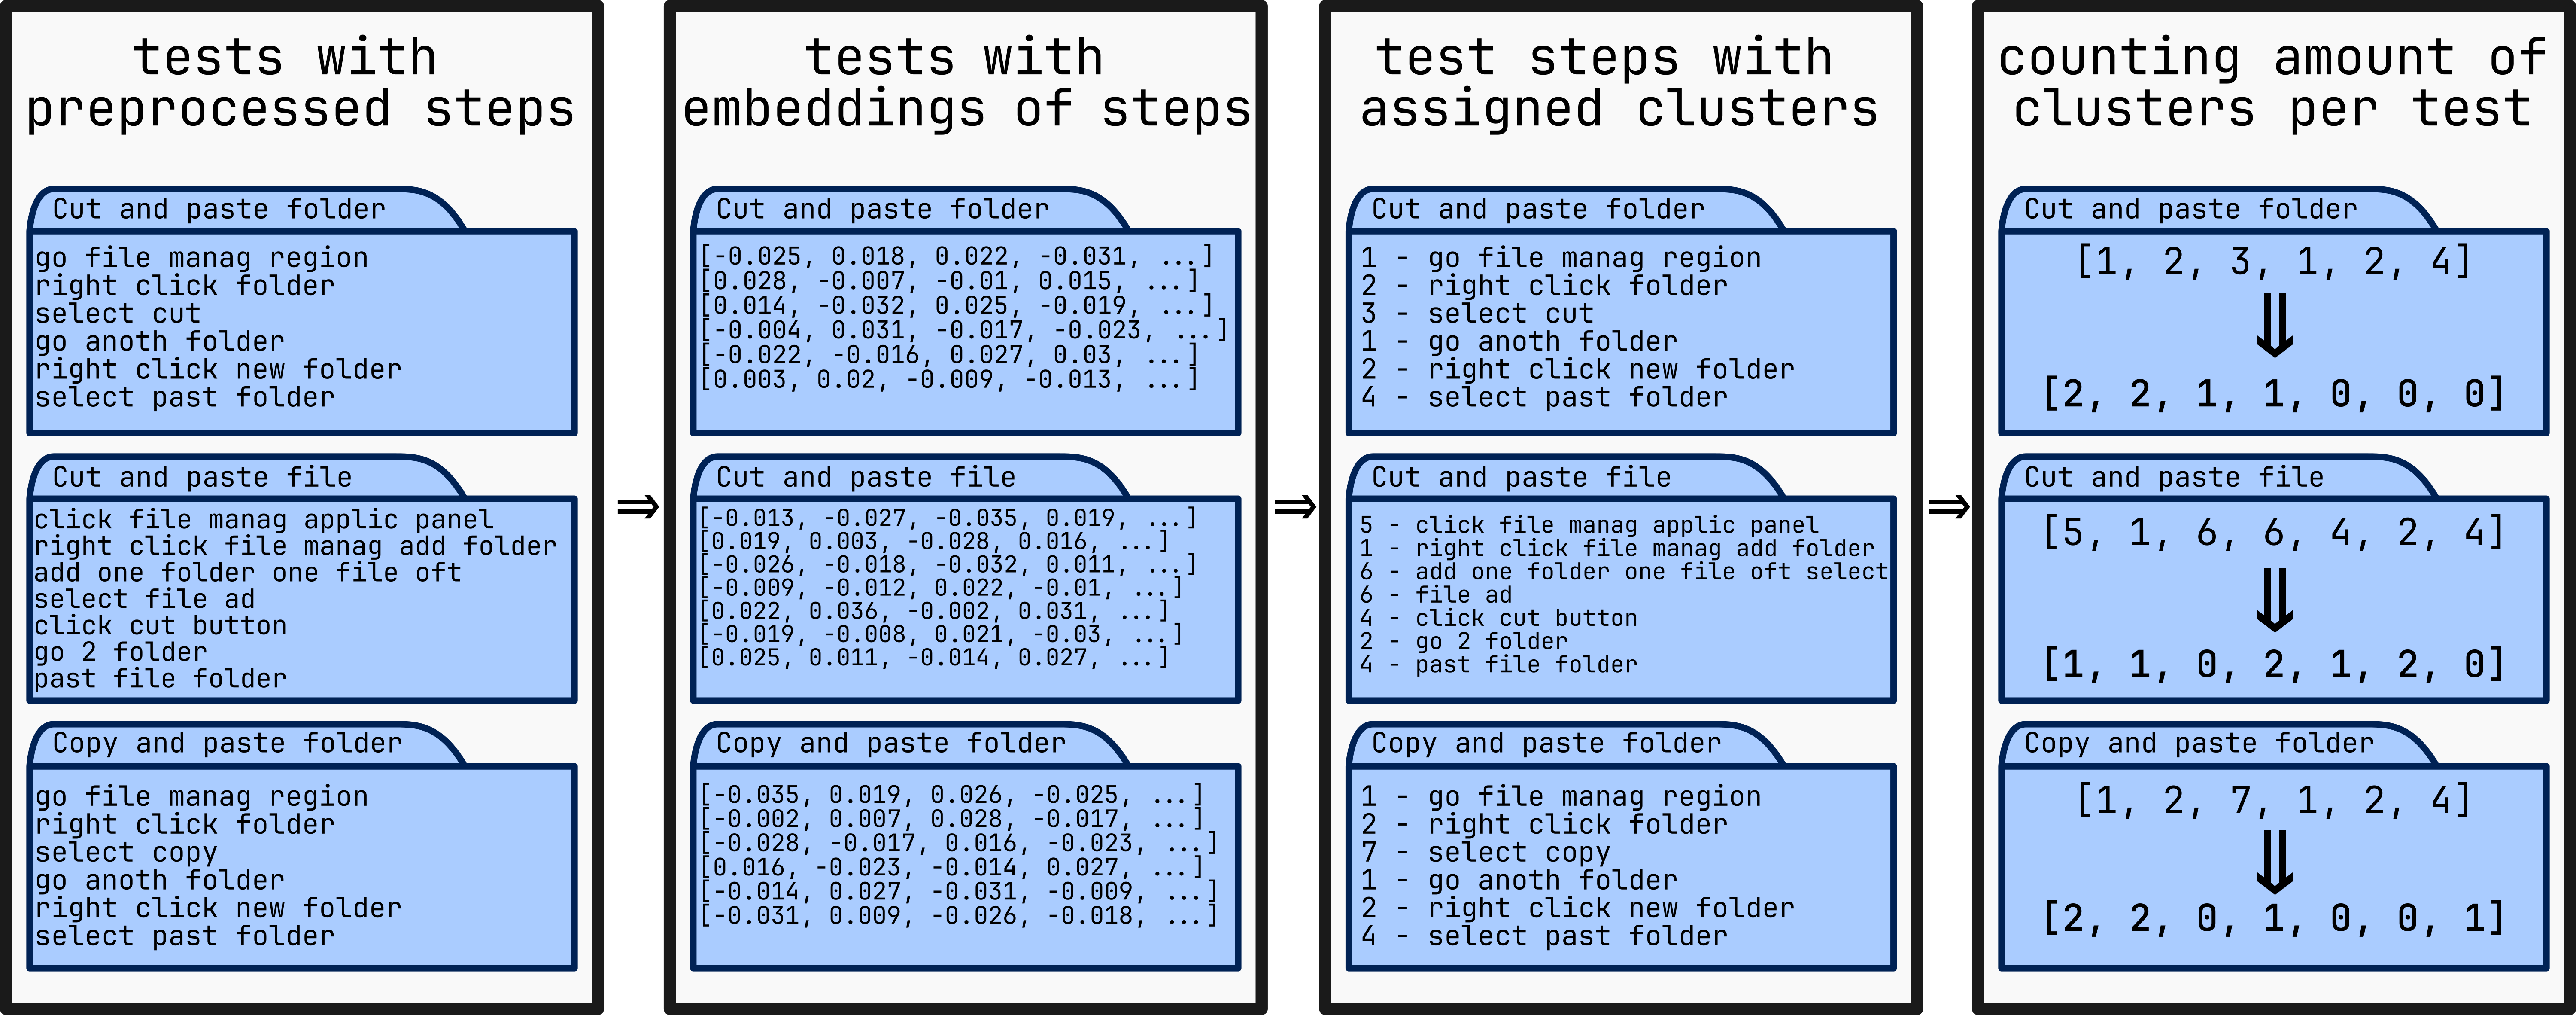
\includegraphics[width=0.9\paperwidth]{figures/getting_representation_for_tests.png}%
}
\caption{Getting a vector representation for each test}

\end{figure}


These Vectors now represent our tests in a mathematical way, which, as mentioned earlier, we want to compare the tests with other tests.
To achieve this, we cluster again after these vectors and as we want to select \emph{n} dissimilar test cases, we cluster with KMeans to cluster the tests into \emph{n} clusters.

After that, we have \emph{n} clusters of test cases from which we then randomly select one test each. This will be our test selection.
